% !TeX program = xelatex
\documentclass[a4paper, 8pt]{extarticle}
\usepackage[total={210mm,279.4mm}, width=170mm, top=20mm, left=20mm, right=20mm, bottom=20mm]{geometry}
\newcommand{\template}[1]{}

\newlength{\headerColumn}
\setlength{\headerColumn}{2.5cm}
\newlength{\firstColumn}
\setlength{\firstColumn}{2cm}
\newlength{\lastColumn}
\setlength{\lastColumn}{6cm}

%A Few Useful Packages
\usepackage[german, english]{babel}
\selectlanguage{\template{["settings"]["currentLanguage"]["en"]}}
\usepackage{calc}
\usepackage{tabularx}
\usepackage[document]{ragged2e}
\usepackage{lipsum}
\usepackage{multirow}
\usepackage{marvosym}
\usepackage{fontspec} 					%for loading fonts
\usepackage{xunicode,xltxtra,url,parskip} 	%other packages for formatting
\RequirePackage{color,graphicx}
\usepackage[usenames,dvipsnames]{xcolor}
%\usepackage[big]{layaureo} 				%better formatting of the A4 page
% an alternative to Layaureo can be ** \usepackage{fullpage} **
\usepackage{supertabular} 				%for Grades
\usepackage{titlesec}					%custom \section
\usepackage{colortbl}
\usepackage{xcolor}

%Setup hyperref package, and colours for links
\usepackage{hyperref}
\definecolor{linkcolor}{rgb}{0,0.0,0.0}
\hypersetup{colorlinks,breaklinks,urlcolor=linkcolor, linkcolor=linkcolor, filecolor=linkcolor, linkbordercolor=linkcolor, urlbordercolor=linkcolor, filebordercolor=linkcolor}
\makeatletter
\Hy@AtBeginDocument{%
	\def\@pdfborder{0 0 0}% Overrides border definition set with colorlinks=true
	\def\@pdfborderstyle{/S/U/W 0.5}% Overrides border style set with colorlinks=true
	% Hyperlink border style will be underline of width 1pt
}
\makeatother

%FONTS
\hyphenchar\font=-1
\hyphenpenalty=1000
\exhyphenpenalty=1000
\defaultfontfeatures{Mapping=tex-text}
\linespread{1.3}
%\setmainfont[SmallCapsFont = Fontin SmallCaps]{Fontin}
%%% modified for Karol Kozioł for ShareLaTeX use
%\setmainfont[
%SmallCapsFont = Fontin-SmallCaps.otf,
%BoldFont = Fontin-Bold.otf,
%ItalicFont = Fontin-Italic.otf
%]
%{Fontin.otf}
%%%
\setmainfont[
BoldFont = cmunrb.otf,
ItalicFont = cmunsl.otf,
BoldItalicFont = cmunbl.otf
]{cmunrm.otf}

%CV Sections inspired by:
%http://stefano.italians.nl/archives/26
\titleformat{\section}{\Large\bfseries\raggedright}{}{0em}{}[\titlerule]
\titlespacing{\section}{0pt}{3pt}{3pt}
%Tweak a bit the top margin
%\addtolength{\voffset}{-1.3cm}

%-------------WATERMARK TEST [**not part of a CV**]---------------
\usepackage[absolute]{textpos}
%\usepackage{fancyhdr}

\setlength{\TPHorizModule}{30mm}
\setlength{\TPVertModule}{\TPHorizModule}
\textblockorigin{2mm}{0.65\paperheight}
\setlength{\parindent}{0pt}
\setlength{\parskip}{1em}
\newlength\savedwidth
\definecolor{hbar}{HTML}{808080}
\newcommand\whline[1]{\arrayrulecolor{hbar}\noalign{\global\savedwidth\arrayrulewidth\global\arrayrulewidth 2pt}%
\cline{#1}
\noalign{\global\arrayrulewidth\savedwidth}}
%\renewcommand{\textbf}[1]{\scalebox{0.8}[1]{\bfseries #1}}
\usepackage{scrpage2}
\pagestyle{scrheadings} % non-numbered pages

\ihead[]{}
\chead[]{}
\ohead[]{}
\ifoot[]{}
\cfoot[\template{["personalInformation"]["firstName"]} \template{["personalInformation"]["middleName"]} \template{["personalInformation"]["lastName"]}]{\template{["personalInformation"]["firstName"]} \template{["personalInformation"]["middleName"]} \template{["personalInformation"]["lastName"]}}
\ofoot[\pagemark]{\pagemark}
%--------------------BEGIN DOCUMENT----------------------
\begin{document}
\hyphenation{Bachelor-arbeit Master-arbeit Programmier-sprachen Frei-willigen-arbeit Doktor-arbeit}
%WATERMARK TEST [**not part of a CV**]---------------
%\font\wm=''Baskerville:color=787878'' at 8pt
%\font\wmweb=''Baskerville:color=FF1493'' at 8pt
%{\wm
%	\begin{textblock}{1}(0,0)
%		\rotatebox{-90}{\parbox{500mm}{
%			Typeset by Alessandro Plasmati with \XeTeX\  \today\ for
%			{\wmweb \href{http://www.aleplasmati.comuv.com}{aleplasmati.comuv.com}}
%		}
%	}
%	\end{textblock}
%}



\font\fb=''[cmr10]'' %for use with \LaTeX command

%--------------------TITLE-------------
\par{\Huge \bfseries \scalebox{1.2}[1.2]{Curriculum Vitae [\template{["personalInformation"]["firstName"]} \template{["personalInformation"]["middleName"]} \template{["personalInformation"]["lastName"]}]}
\bigskip\par}

%--------------------SECTIONS-----------------------------------
%Section: Personal Data

\begin{tabular}{p{\headerColumn}p{2.6cm}p{21mm}p{\textwidth-\headerColumn-2.6cm-21mm-16mm}}
	\whline{2-4}\\[0.1mm]
	\multirow[t]{7}{\headerColumn}{\Large\bfseries\raggedleft \template{["personalInformation"]["_name"]["en"]}}
	&
	\multirow{7}{2.6cm}{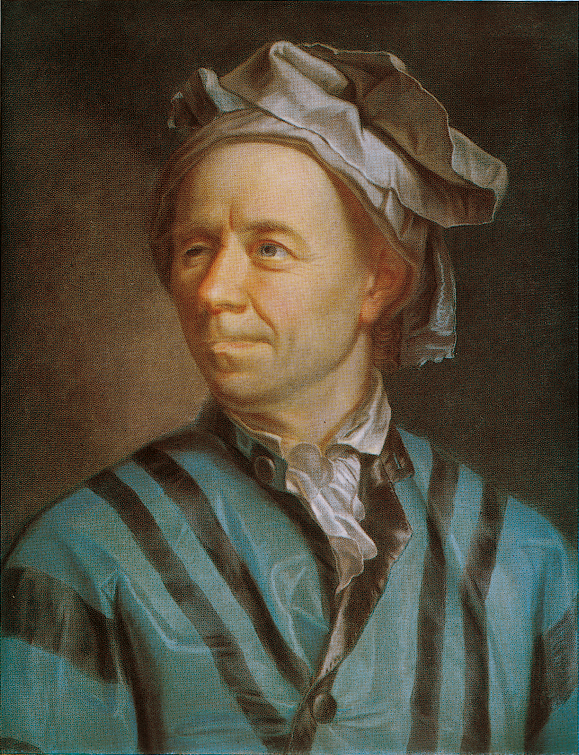
\includegraphics[width=2.6cm, height=3.466cm]{img/mypics/Leonhard_Euler_by_Handmann.png}}
	&
	 \raggedleft \template{["personalInformation"]["birthDate"]["_name"]["en"]}:& \textbf{\template{["personalInformation"]["birthDate"]["en"]}} \\
	 &&\raggedleft \template{["personalInformation"]["nationality"]["_name"]["en"]}:&  \textbf{\template{["personalInformation"]["nationality"]["en"]}}\\
	 &&\raggedleft \template{["personalInformation"]["address"]["_name"]["en"]}:& \textbf{\template{["personalInformation"]["address"]["en"]}} \\
	 &&\raggedleft \template{["personalInformation"]["email"]["_name"]["en"]}:& \textbf{\href{\template{["personalInformation"]["email"]["address"]}}{\template{["personalInformation"]["email"]["address"]}}}\\
	 &&\raggedleft \template{["personalInformation"]["phone"]["_name"]["en"]}:& \textbf{\template{["personalInformation"]["phone"]["number"]}}\\
	 &&\raggedleft Github:& \textbf{\href{\template{["personalInformation"]["links"]["github"]}}{\template{["personalInformation"]["links"]["github"]}}}\\
	 &&\raggedleft LinkedIn:& \textbf{\href{\template{["personalInformation"]["links"]["linkedIn"]}}{\template{["personalInformation"]["links"]["linkedIn"]}}}\\[5mm]
\end{tabular}
\vskip 0mm
\begin{tabular}{p{\headerColumn}p{\textwidth-\headerColumn-8mm}}
	\whline{2-2}&\\
	\Large\bfseries\raggedleft \template{["introduction"]["_name"]["en"]}&
	\par{\template{["introduction"]["en"]}}
\end{tabular}
%\extrarowheight=0.15cm
\vskip 0mm
%Section: Works
\begin{tabular}[t]{p{\headerColumn}p{\textwidth-\headerColumn-8mm}}
	\whline{2-2}&\\
	\Large\bfseries\raggedleft \template{["works"]["_name"]["en"]}&
\begin{tabular}[t]{p{\firstColumn}p{\textwidth-\firstColumn-\headerColumn-16mm}}
	
	\template{LOOP "i" ["works"]["list"]}
		\multirow[t]{3}{\firstColumn}{ \raggedleft \large\textbf{\template{["works"]["list"][i]["kind"]["en"]}}} & \textbf{\href{\template{["works"]["list"][i]["link"]}}{\template{["works"]["list"][i]["title"]}}}\\
		&\par{\textbf{\template{["works"]["_name"]["supervisors"]["en"]}:}
		\template{LOOP "j" ["works"]["list"][i]["supervisors"]}
			\href{\template{["works"]["list"][i]["supervisors"][j]["link"]}}{\template{["works"]["list"][i]["supervisors"][j]["name"]}},
		\template{ENDLOOP "j"}}\\
		&\par{\textit{\template{["works"]["list"][i]["description"]["simple"]["en"]}}}\\
		&\par{\textbf{Tech-Stack}:
		\template{LOOP "j" ["works"]["list"][i]["techStack"]}
			\template{["works"]["list"][i]["techStack"][j]},
		\template{ENDLOOP "j"}}\\
	\template{ENDLOOP "i"}
\end{tabular}
\end{tabular}

%Section: Education
\begin{tabular}[t]{p{\headerColumn}p{\textwidth-\headerColumn-8mm}}
	\whline{2-2}&\\
	\Large\bfseries\raggedleft \template{["education"]["_name"]["en"]}&
\begin{tabular}[t]{p{\firstColumn}p{\textwidth-\lastColumn-\firstColumn-\headerColumn-16mm}p{\lastColumn}}
\template{LOOP "i" ["education"]["list"]}
	\raggedleft \template{["education"]["list"][i]["from"]} - \template{["education"]["list"][i]["to"]} & \textbf{\template{["education"]["list"][i]["title"]["en"]}} & \href{\template{["education"]["list"][i]["organization"]["link"]}}{\template{["education"]["list"][i]["organization"]["en"]} \template{["education"]["list"][i]["organization"]["abbreviation"]}}\\
\template{ENDLOOP "i"}
\end{tabular}
\end{tabular}

%Section: Work Experience
\begin{tabular}[t]{p{\headerColumn}p{\textwidth-\headerColumn-8mm}}
	\whline{2-2}&\\
	\Large\bfseries\raggedleft \template{["experience"]["_name"]["en"]}&
\begin{tabular}[t]{p{\firstColumn}p{\textwidth-\firstColumn-\lastColumn-\headerColumn-16mm}p{\lastColumn}}
	\template{LOOP "i" ["experience"]["list"]}
		\raggedleft \template{["experience"]["list"][i]["from"]} - \template{["experience"]["list"][i]["to"]} & \textbf{\template{["experience"]["list"][i]["title"]["en"]}} & \href{\template{["experience"]["list"][i]["company"]["link"]}}{\template{["experience"]["list"][i]["company"]["name"]}}\\
		&\multicolumn{2}{p{\textwidth-\firstColumn-\headerColumn-16mm}}{\par{\textit{\template{["experience"]["list"][i]["description"]["en"]}}}}\\
		&\multicolumn{2}{p{\textwidth-\firstColumn-\headerColumn-16mm}}{\par{\textbf{Tech-Stack:}
		\template{LOOP "j" ["experience"]["list"][i]["techStack"]}
			\template{["experience"]["list"][i]["techStack"][j]},
		\template{ENDLOOP "j"}
		}}\\
	\template{ENDLOOP "i"}
\end{tabular}
\end{tabular}

\begin{tabular}[t]{p{\headerColumn}p{\textwidth-\headerColumn-8mm}}
	\whline{2-2}&\\
	\Large\bfseries\raggedleft \template{["skills"]["_name"]["en"]}&
\begin{tabular}[t]{p{\firstColumn}p{\textwidth-\firstColumn-\lastColumn-\headerColumn-16mm}p{\lastColumn}}
	\multirow[t]{2}{\firstColumn}{\raggedleft \textbf{\template{["skills"]["languages"]["_name"]["en"]}}}
	 & \raggedleft
	\template{LOOP "i" ["skills"]["languages"]["firstLanguage"]["names"]["en"]}
		\template{["skills"]["languages"]["firstLanguage"]["names"]["en"][i]},
	\template{ENDLOOP "i"}
	& \template{["skills"]["languages"]["firstLanguage"]["en"]}\\
	& \raggedleft \template{LOOP "i" ["skills"]["languages"]["fluent"]["names"]["en"]}
	\template{["skills"]["languages"]["fluent"]["names"]["en"][i]},
	\template{ENDLOOP "i"}
	& \template{["skills"]["languages"]["fluent"]["en"]}\\
	\cline{2-3} 
	\multirow[t]{3}{\firstColumn}{
		\hspace{0pt}\raggedleft \textbf{\template{["skills"]["programmingLanguages"]["_name"]["en"]}}
	} & \raggedleft
	\template{LOOP "i" ["skills"]["programmingLanguages"]["skilled"]["list"]}
		\template{["skills"]["programmingLanguages"]["skilled"]["list"][i]},
	\template{ENDLOOP "i"}
	& \template{["skills"]["programmingLanguages"]["skilled"]["en"]}\\
	& \raggedleft \template{LOOP "i" ["skills"]["programmingLanguages"]["experienced"]["list"]}
	\template{["skills"]["programmingLanguages"]["experienced"]["list"][i]},
	\template{ENDLOOP "i"}
	& \template{["skills"]["programmingLanguages"]["experienced"]["en"]}\\
	& \raggedleft \template{LOOP "i" ["skills"]["programmingLanguages"]["basicKnowledge"]["list"]}
	\template{["skills"]["programmingLanguages"]["basicKnowledge"]["list"][i]},
	\template{ENDLOOP "i"}
	& \template{["skills"]["programmingLanguages"]["basicKnowledge"]["en"]}\\
	\cline{2-3} 
	\multirow[t]{2}{\firstColumn}{\raggedleft \textbf{\template{["skills"]["technologies"]["_name"]["en"]}}} & \raggedleft
	\template{LOOP "i" ["skills"]["technologies"]["skilled"]["list"]}
	\template{["skills"]["technologies"]["skilled"]["list"][i]},
	\template{ENDLOOP "i"}
	& \template{["skills"]["technologies"]["skilled"]["en"]}\\
	&\raggedleft \template{LOOP "i" ["skills"]["technologies"]["basicKnowledge"]["list"]}
	\template{["skills"]["technologies"]["basicKnowledge"]["list"][i]},
	\template{ENDLOOP "i"}
	& \template{["skills"]["technologies"]["basicKnowledge"]["en"]}\\
\end{tabular}
\end{tabular}


%Section: Volunteer Work

\begin{tabular}[t]{p{\headerColumn}p{\textwidth-\headerColumn-8mm}}
	\whline{2-2}&\\
	\hspace{0pt}\Large\bfseries\raggedleft \template{["volunteerWork"]["_name"]["en"]}&
\begin{tabular}[t]{p{\firstColumn}p{\textwidth-\firstColumn-\lastColumn-\headerColumn-16mm}p{\lastColumn}}
\template{LOOP "i" ["volunteerWork"]["list"]}
	\raggedleft \template{["volunteerWork"]["list"][i]["from"]} - \template{["volunteerWork"]["list"][i]["to"]} & \template{["volunteerWork"]["list"][i]["title"]["en"]} & \template{["volunteerWork"]["list"][i]["description"]["en"]}\\
\template{ENDLOOP "i"}
\end{tabular}
\end{tabular}


\end{document}
